\section{Hardware-in-the-Loop Architecture}

The successful implementation of the prototype relies on the seamless integration of the mechanical hardware
with the control software. To bridge the theoretical environment (MATLAB/Simulink) with the physical reality, a
Hardware-in-the-Loop (HIL) architecture was established. This approach allows the complex kinematic algorithms
to run on the host PC, while a dedicated embedded bridge manages the low-level communication with the distributed
actuator network.


\subsubsection{Physical Assembly}

The mechanical structure of the limb was realized through additive manufacturing (3D printing) using the CAD
models developed during the design phase. The structural links (Coxa, Femur, Tibia) were printed in PLA to
ensure an optimal stiffness-to-weight ratio.

These components were assembled with the three newly designed custom actuator modules described in Chapter
\ref{ch:servomotor} (see Figure \ref{fig:limb_assembly}). A critical design feature introduced in this assembly is
the axis extension mechanism. To mitigate the radial stress on the servo output shaft an idler bearing was integrated
into the frame opposite to the motor shaft. This configuration effectively creates a simply supported beam structure,
significantly increasing mechanical stability.

\begin{figure}[htbp]
    \centering
    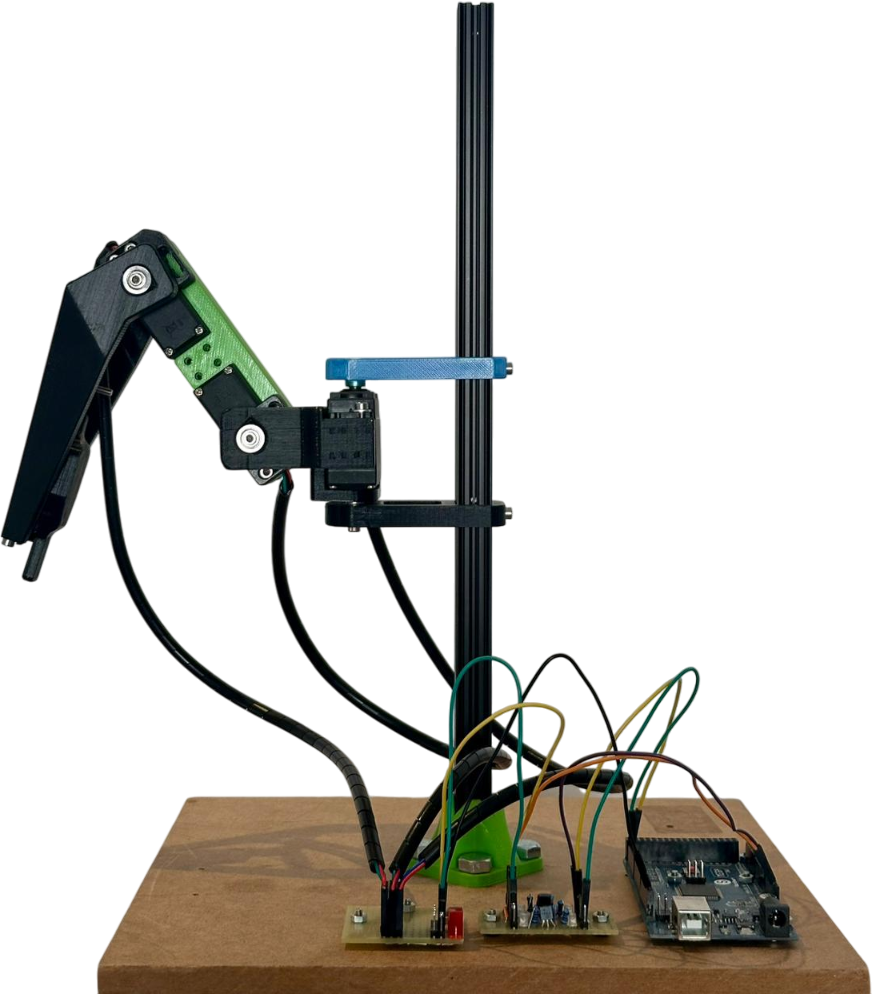
\includegraphics[width=0.88\textwidth]{images/limb_assembly.png}
    \caption{Mechanical Assembly of the Prototype Limb.}
    \label{fig:limb_assembly}
\end{figure}

With the exception of the custom actuator housings and fasteners, the physical limb geometrically coincides perfectly
with the numerical model used in the simulations (Section \ref{sc:simulation}), providing a first visual
confirmation of the prototype's fidelity.


\subsubsection{Simulink/Arduino Control Environment}

The Simulink model, originally developed for pure digital simulation, acts as the High-Level Controller. The
"Leg Model (Plant)" block used in Chapter \ref{ch:model} is replaced by a Serial Interface Block. This modified
control scheme (Figure \ref{fig:hil_scheme}) operates as follows:

\begin{enumerate}
    \item Generation and Transmission: The Path Planner and Inverse Kinematics blocks generate the reference
        joint angles $q_d$ in real-time. These references are quantized and transmitted via USB-Serial to the
        microcontroller bridge.
    \item Hardware Bridge: The interface between the host PC and the actuator network is managed by an Arduino
        board (Arduino Mega 2560). The firmware sketch, parses the UART data and forwards the position setpoints
        to the actuator network via $\text{I}^2\text{C}$ bus. Immediately after it queries their current position
        (also via $\text{I}^2\text{C}$). Then the received data ($q_{hw}$) is transmitted back to Simulink.
    \item Feedback Loop: After the return packet containing the measured joint angles $q_{hw}$ arrives, the
        feedback data is fed into the Forward Kinematics block to reconstruct the actual end-effector position
        $p_{hw}$ for performance analysis.
\end{enumerate}

\begin{figure}[htbp]
    \centering
    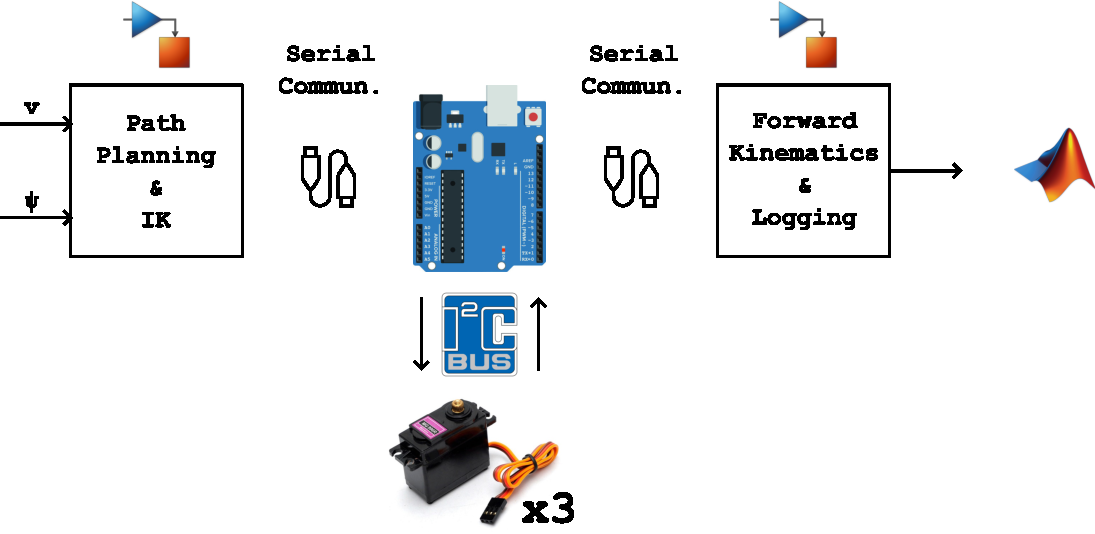
\includegraphics[width=0.9\textwidth]{images/hil.pdf}
    \caption{Block Diagram of the Hardware-in-the-Loop Control Architecture.}
    \label{fig:hil_scheme}
\end{figure}


\subsubsection{Experimental Protocol}

To ensure a rigorous validation, the experimental setup is designed to strictly mirror the conditions of the
digital simulation presented in Chapter \ref{ch:model}. The reference input for the physical limb is the exact
same $C^2$ continuous gait trajectory derived in Section \ref{sec:trajectory}.

The real-time control chain operates at a fixed update frequency of $100\,\text{Hz}$ ($\Delta t = 10\,\text{ms}$).
In each cycle, the Simulink High-Level Controller samples the continuous trajectory, computes the inverse
kinematics solution $q_d$, and transmits the packet to the embedded bridge. Synchronously, the actual joint
positions $q_{hw}$ are acquired from the actuators and logged.

The primary objective of this experiment is to quantify the \textit{Sim-to-Real} gap by overlaying the
experimental data on the simulation results.